% MeanFlow StormCast -- training step workflow.
% Notation matches the thesis formula deck (X_{t-1} HighRes state,
% M_t = F_xi(...) regression mean, R_t = X_t - M_t residual target).
\documentclass[border=14pt]{standalone}
% Shared MeanFlow-StormCast workflow style.
% Palette = thesis viridis convention (mirrors make_method_figures.py /
% build_formulas.py): borders at viridis ramp positions, fills tinted to white.
\usepackage{amsmath,amssymb,bm}
\usepackage{xcolor}
\usepackage{tikz}
\usetikzlibrary{positioning,arrows.meta,calc,fit,backgrounds,shapes.geometric}

% --- viridis-sampled palette (border / light fill) -------------------------
\definecolor{cFrozen}{HTML}{481D6F}\definecolor{cFrozenF}{HTML}{EDE8F1} % frozen nets
\definecolor{cSamp}{HTML}{355F8D}\definecolor{cSampF}{HTML}{EBEFF4}     % flow-space / sampler
\definecolor{cFlow}{HTML}{287D8E}\definecolor{cFlowF}{HTML}{E9F2F4}     % trained MeanFlow net
\definecolor{cLoss}{HTML}{1E9C89}\definecolor{cLossF}{HTML}{E9F5F3}     % loss terms
\definecolor{cOut}{HTML}{26AD81}\definecolor{cOutF}{HTML}{E9F7F2}       % composition / output
\definecolor{cData}{HTML}{737373}\definecolor{cDataF}{HTML}{F1F1F1}     % data / tensors
\definecolor{cEdge}{HTML}{5A5A5A}

\tikzset{
  base/.style   ={rounded corners=3pt, draw, line width=0.9pt, align=center,
                  inner sep=5pt, font=\small, text=black!88},
  data/.style   ={base, draw=cData,   fill=cDataF},
  frozen/.style ={base, draw=cFrozen, fill=cFrozenF},
  trained/.style={base, draw=cFlow,   fill=cFlowF},
  sampler/.style={base, draw=cSamp,   fill=cSampF},
  loss/.style   ={base, draw=cLoss,   fill=cLossF},
  output/.style ={base, draw=cOut,    fill=cOutF},
  total/.style  ={base, draw=black!80, fill=black!7, line width=1.1pt},
  flow/.style   ={-{Stealth[length=2.4mm]}, line width=0.9pt, draw=cEdge},
  thin flow/.style={-{Stealth[length=2.0mm]}, line width=0.7pt, draw=cData},
  feedback/.style={-{Stealth[length=2.4mm]}, line width=0.9pt, draw=cData,
                  dashed, dash pattern=on 4pt off 3pt},
  emaedge/.style={-{Stealth[length=2.2mm]}, line width=0.8pt, draw=cData,
                  dashed, dash pattern=on 3pt off 2.5pt},
  container/.style={rounded corners=6pt, draw=black!35, line width=0.8pt,
                  dashed, dash pattern=on 3pt off 2.5pt, fill=black!2,
                  inner sep=8pt},
  ttl/.style    ={font=\bfseries\large, text=black!85},
  sub/.style    ={font=\itshape\footnotesize, text=black!55},
  lg/.style     ={font=\scriptsize, text=black!60},
}

% legend swatch helper
\newcommand{\swatch}[2]{%
  \tikz[baseline=-0.5ex]\node[rounded corners=1.5pt, draw=#1, fill=#1!12,
    line width=0.9pt, minimum width=3.4mm, minimum height=2.6mm, inner sep=0]{};\;#2}

\begin{document}
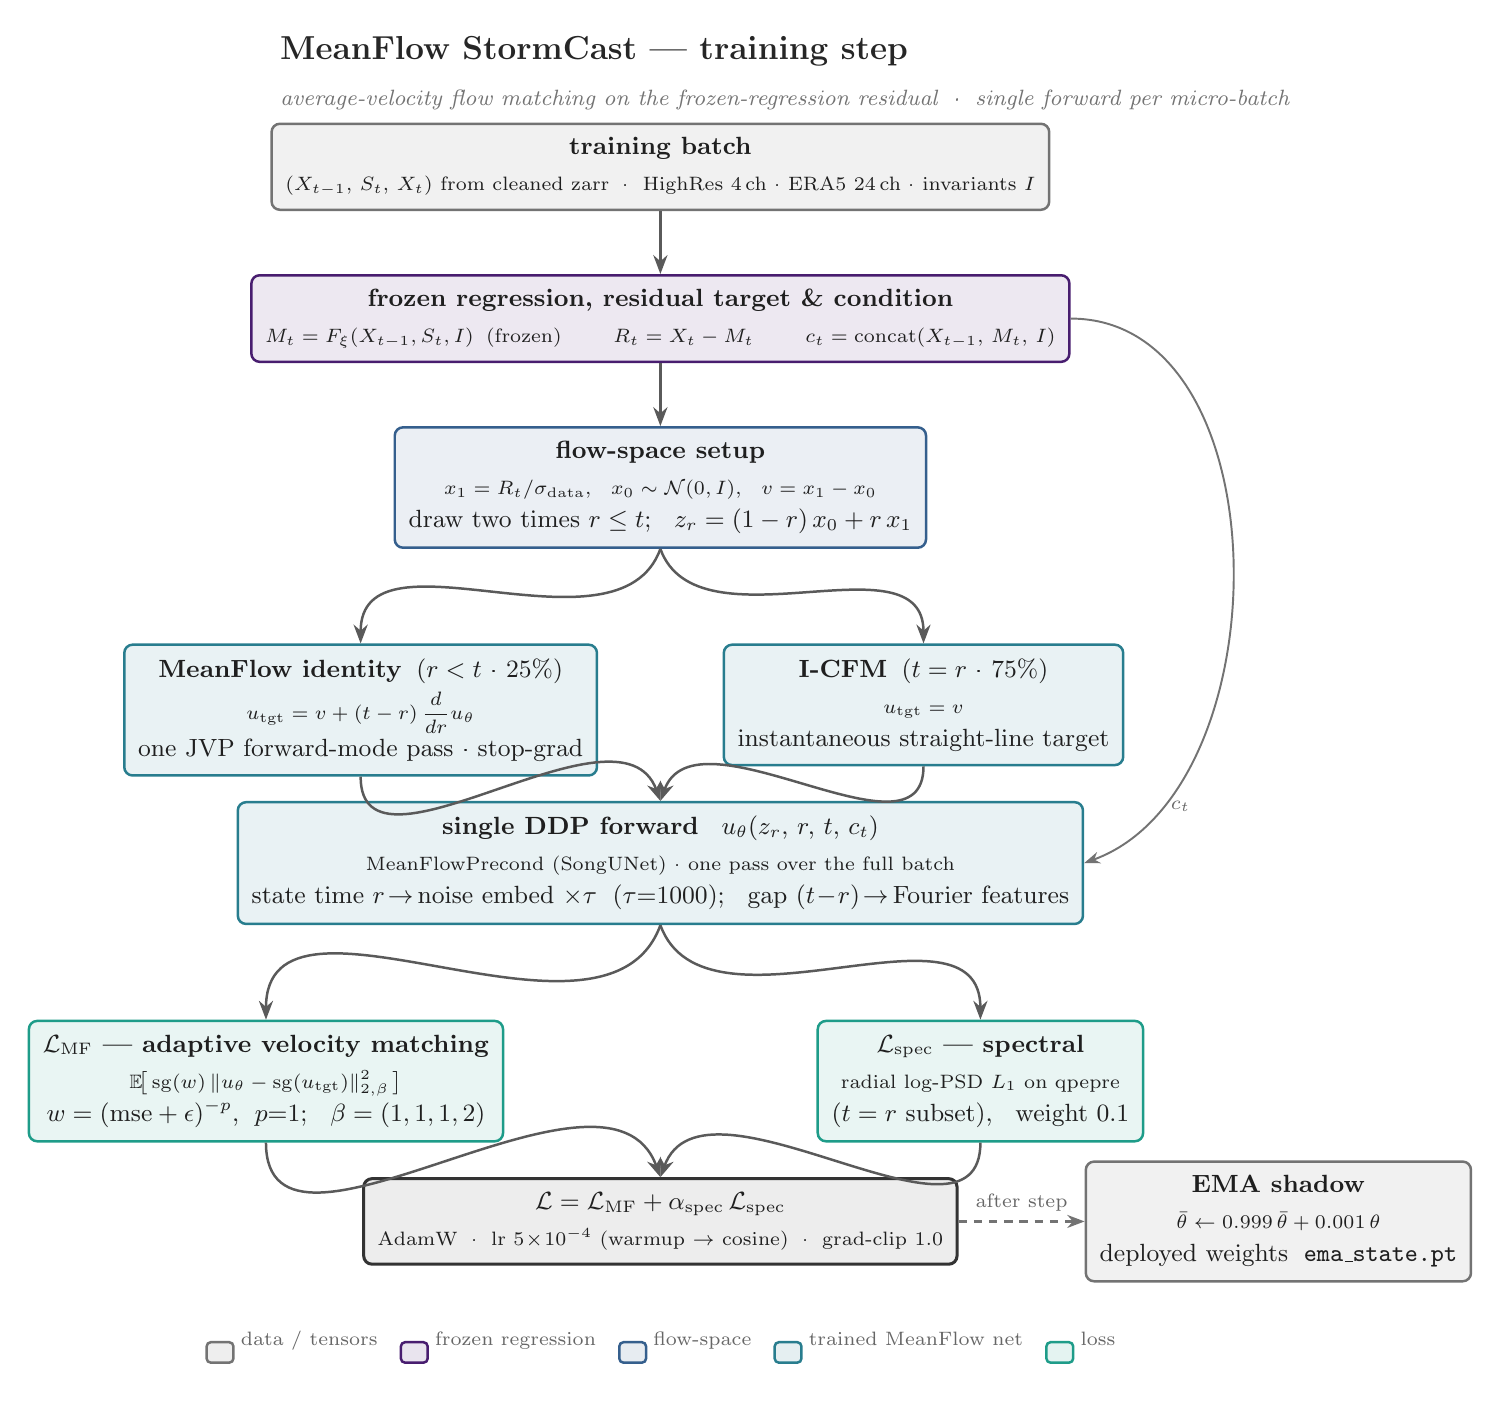
\begin{tikzpicture}[node distance=8mm]

  % ---- title ----
  \node[ttl] (title) at (0,0) {MeanFlow StormCast --- training step};
  \node[sub, below=0.5mm of title.south west, anchor=north west]
    {average-velocity flow matching on the frozen-regression residual \;·\; single forward per micro-batch};

  % ---- batch ----
  \node[data, below=9mm of title.west, anchor=north west] (batch)
    {\textbf{training batch}\\[2pt]\scriptsize $(X_{t-1},\,S_t,\,X_t)$ from cleaned zarr \;·\; HighRes 4\,ch · ERA5 24\,ch · invariants $I$};

  % ---- frozen regression + residual target + condition ----
  \node[frozen, below=of batch] (cond)
    {\textbf{frozen regression, residual target \& condition}\\[2pt]\scriptsize $M_t = F_\xi(X_{t-1},S_t,I)$\;\;(frozen) \qquad $R_t = X_t - M_t$ \qquad $c_t = \mathrm{concat}(X_{t-1},\,M_t,\,I)$};

  % ---- flow-space setup ----
  \node[sampler, below=of cond] (flow)
    {\textbf{flow-space setup}\\[2pt]\scriptsize $x_1 = R_t/\sigma_{\mathrm{data}}$,\;\; $x_0\sim\mathcal N(0,I)$,\;\; $v = x_1-x_0$\\[1pt]draw two times $r\le t$;\;\; $z_r = (1-r)\,x_0 + r\,x_1$};

  % ---- branch: MeanFlow identity vs I-CFM ----
  \node[trained, below left=12mm and -26mm of flow] (mf)
    {\textbf{MeanFlow identity}\;\;($r<t$ · 25\%)\\[2pt]\scriptsize $u_{\mathrm{tgt}} = v + (t-r)\,\dfrac{d}{dr}u_\theta$\\[1pt]one JVP forward-mode pass · stop-grad};
  \node[trained, below right=12mm and -26mm of flow] (icfm)
    {\textbf{I-CFM}\;\;($t=r$ · 75\%)\\[2pt]\scriptsize $u_{\mathrm{tgt}} = v$\\[1pt]instantaneous straight-line target};

  % ---- single student forward ----
  \node[trained, below=32mm of flow] (fwd)
    {\textbf{single DDP forward}\;\; $u_\theta(z_r,\,r,\,t,\,c_t)$\\[2pt]\scriptsize MeanFlowPrecond (SongUNet) · one pass over the full batch\\[1pt]state time $r\!\to\!$ noise embed $\times\tau$ \;($\tau{=}1000$);\;\; gap $(t\!-\!r)\!\to\!$ Fourier features};

  % ---- losses ----
  \node[loss, below left=12mm and -34mm of fwd] (lflow)
    {\textbf{$\mathcal L_{\mathrm{MF}}$ --- adaptive velocity matching}\\[2pt]\scriptsize $\mathbb E\!\big[\,\mathrm{sg}(w)\,\lVert u_\theta - \mathrm{sg}(u_{\mathrm{tgt}})\rVert_{2,\beta}^2\,\big]$\\[1pt]$w=(\mathrm{mse}+\epsilon)^{-p}$,\; $p{=}1$;\;\; $\beta=(1,1,1,2)$};
  \node[loss, below right=12mm and -34mm of fwd] (lspec)
    {\textbf{$\mathcal L_{\mathrm{spec}}$ --- spectral}\\[2pt]\scriptsize radial log-PSD $L_1$ on qpepre\\[1pt]($t=r$ subset),\;\; weight $0.1$};

  % ---- total + optimizer ----
  \node[total, below=32mm of fwd] (total)
    {\textbf{$\mathcal L = \mathcal L_{\mathrm{MF}} + \alpha_{\mathrm{spec}}\,\mathcal L_{\mathrm{spec}}$}\\[2pt]\scriptsize AdamW \;·\; lr $5\!\times\!10^{-4}$ (warmup $\to$ cosine) \;·\; grad-clip $1.0$};

  % ---- EMA side ----
  \node[data, right=16mm of total] (ema)
    {\textbf{EMA shadow}\\[2pt]\scriptsize $\bar\theta \leftarrow 0.999\,\bar\theta + 0.001\,\theta$\\[1pt]deployed weights \;\texttt{ema\_state.pt}};

  % ---- edges ----
  \draw[flow] (batch) -- (cond);
  \draw[flow] (cond) -- (flow);
  \draw[flow] (flow.south) to[out=-110,in=90] (mf.north);
  \draw[flow] (flow.south) to[out=-70,in=90] (icfm.north);
  \draw[flow] (mf.south) to[out=-90,in=110] (fwd.north);
  \draw[flow] (icfm.south) to[out=-90,in=70] (fwd.north);
  \draw[flow] (fwd.south) to[out=-110,in=90] (lflow.north);
  \draw[flow] (fwd.south) to[out=-70,in=90] (lspec.north);
  \draw[flow] (lflow.south) to[out=-90,in=110] (total.north);
  \draw[flow] (lspec.south) to[out=-90,in=70] (total.north);
  \draw[emaedge] (total.east) -- (ema.west) node[midway,above,lg]{after step};

  % conditioning side-channel into the student forward
  \draw[thin flow] (cond.east) to[out=0,in=20]
        node[pos=0.85,right,lg]{$c_t$} (fwd.east);

  % ---- legend ----
  \node[lg, anchor=north] at ($(total.south)+(0,-7mm)$)
    {\swatch{cData}{data / tensors}\quad
     \swatch{cFrozen}{frozen regression}\quad
     \swatch{cSamp}{flow-space}\quad
     \swatch{cFlow}{trained MeanFlow net}\quad
     \swatch{cLoss}{loss}};

\end{tikzpicture}
\end{document}
